\begin{center}
	{\scriptsize
		\begin{tabularx}{\textwidth}{p{0.2\textwidth}|p{0.6\textwidth}|p{0.1\textwidth}}
			\caption{Summary of results for achieving the objectives} \label{tab:outcomes_per_objective} \\
			\hline 
			\hline 
			\textbf{Objectives} & 
			\textbf{Results} &
			\textbf{Locations}\\ 
			\hline 
			\endfirsthead
			\multicolumn{3}{c}%
			{\textit{Continued from previous page}} \\
			\hline
			\hline 
			\textbf{Objectives} & 
			\textbf{Results} &
			\textbf{Locations}\\ 
			\hline 
			\endhead
			\hline 
			\multicolumn{3}{r}{\textit{Continued on next page}} \\ 
			\endfoot
			\hline 
			\endlastfoot
			\hline
			
			
			\Paste{GO} & 

			\begin{itemize}
				\item Achieved to gather and create a unique dataset consisting of 500 good and 200 defective beans
				\item Achieved improvisation of the synchronization between the machine vision and embedded system.
			\end{itemize}
			
			& Sec.~\ref{sec:description_dataset} on p.~\pageref{sec:description_dataset} 
			\\ \hline
			
			\Paste{SO1} & 
			\begin{itemize}
				\item Acquired 257 images of Black coffee beans
				\item Gathered 301 images of Broken coffee beans
				\item Gathered 305 images of Dried Cherry coffee beans
				\item Acquired 288 images of Floater coffee beans
				\item Acquired 301 images of Fungus Damage coffee beans
				\item Gathered 1565 images of Good coffee beans
				\item Acquired 345 images of Insect Damage coffee beans
				\item Gathered 320 images of Sour coffee beans
			\end{itemize} & 
			
			Sec.~\ref{sec:description_dataset} on p.~\pageref{sec:description_dataset} 
			\\ \hline
			
			
			\Paste{SO2} & 

			\begin{itemize}
				\item Achieved 22 beans per minute for stage one of the system
			\end{itemize} 
	
			& Sec.~\ref{sec:sorting_speed} on p.~\pageref{sec:sorting_speed}
			\\ \hline
			
			\Paste{SO3} & 
			\begin{itemize}
				\item Achieved 90.07\% testing accuracy in classifying Black coffee beans.
				\item Achieved 90.07\% testing accuracy in identifying Broken coffee beans.
				\item Attained 90.65\% testing accuracy in recognizing Dried Cherry coffee beans.
				\item Recorded 87.78\% testing accuracy in detecting Floater coffee beans.
				\item Achieved 90.65\% testing accuracy in classifying Fungus Damage coffee beans.
				\item Reached  90.07\% testing accuracy in identifying Good coffee beans.
				\item Attained 90.07\% testing accuracy in detecting Insect Damage coffee beans.
				\item Achieved 90.65\% testing accuracy in classifying Sour coffee beans.
				\item Achieved 90.00\% overall testing accuracy of the system.
			\end{itemize} 
			& Sec.~\ref{sec:actual_performance} on p.~\pageref{sec:actual_performance}\\ \hline
			
			
			\Paste{SO4} &
			\begin{itemize}
				\item To achieve 90\% in filtering out less-dense coffee beans
			\end{itemize}
			& 			\\ \hline
			
		\end{tabularx}
	}
\end{center}

\section{Description of the New Custom Dataset}
\label{sec:description_dataset}
\begin{table}[H]
	\centering
	\caption{Class Distribution Summary}
	\label{tab:class_dist_summary}
	\begin{tabular}{l c}
	\toprule
	\textbf{Class Name} & \textbf{Image Count} \\
	\midrule
	Black & 205 \\
	Broken & 203 \\
	Dried Cherry & 206 \\
	Floater & 202 \\
	Fungus Damage & 207 \\
	Good & 604 \\
	Insect Damage & 201 \\
	Sour & 202 \\
	\midrule
	\textbf{Total} & \textbf{2030} \\
	\bottomrule
	\end{tabular}
\end{table}

Table \ref{tab:class_dist_summary} presents the dataset's class distribution after adjustments. The image counts for each category were increased such that the minimum is above 200, with "Good" exceeding 543; for instance, Black has 205 images and Good has 604 images. The table confirms a total of 2,030 images distributed across the eight classes, ensuring a balanced dataset that maintains diversity while meeting the minimum requirements.

\begin{table}[H]
    \centering
    \caption{Dataset Split Summary}
    \label{tab:dataset_split_summary}
    \resizebox{\textwidth}{!}{%
    \begin{tabular}{l c c l}
    \toprule
    \textbf{Split} & \textbf{Percentage} & \textbf{Image Count} & \textbf{Augmentation} \\
    \midrule
    Train & 88\% & 1786 & Original training images are augmented three times \\
    Validation & 8\% & 162 & Non-augmented \\
    Test & 4\% & 82 & Non-augmented \\
    \bottomrule
    \end{tabular}%
    }
\end{table}

Table \ref{tab:dataset_split_summary} outlines the dataset split into training, validation, and test sets. The training set comprises 88\% (1,786 images), while the validation and test sets account for 8\% (162 images) and 4\% (82 images) respectively, with the training images later augmented 3× per image.

\section{Performance of Classification Models on Custom Dataset}
\label{sec:perf_custom_dataset}
Four different classification models, such as EfficientNet, YOLOv8, YOLOv11 and YOLOv12, were benchmarked to determine the most optimal model to be used for the system. Each model was trained using a custom dataset manually gathered by the researchers. In addition, augmentations such as rotation, flip, blur and noise, were applied. 

\subsection{EfficientNetV2S}

\begin{figure}[H]
    \centering
    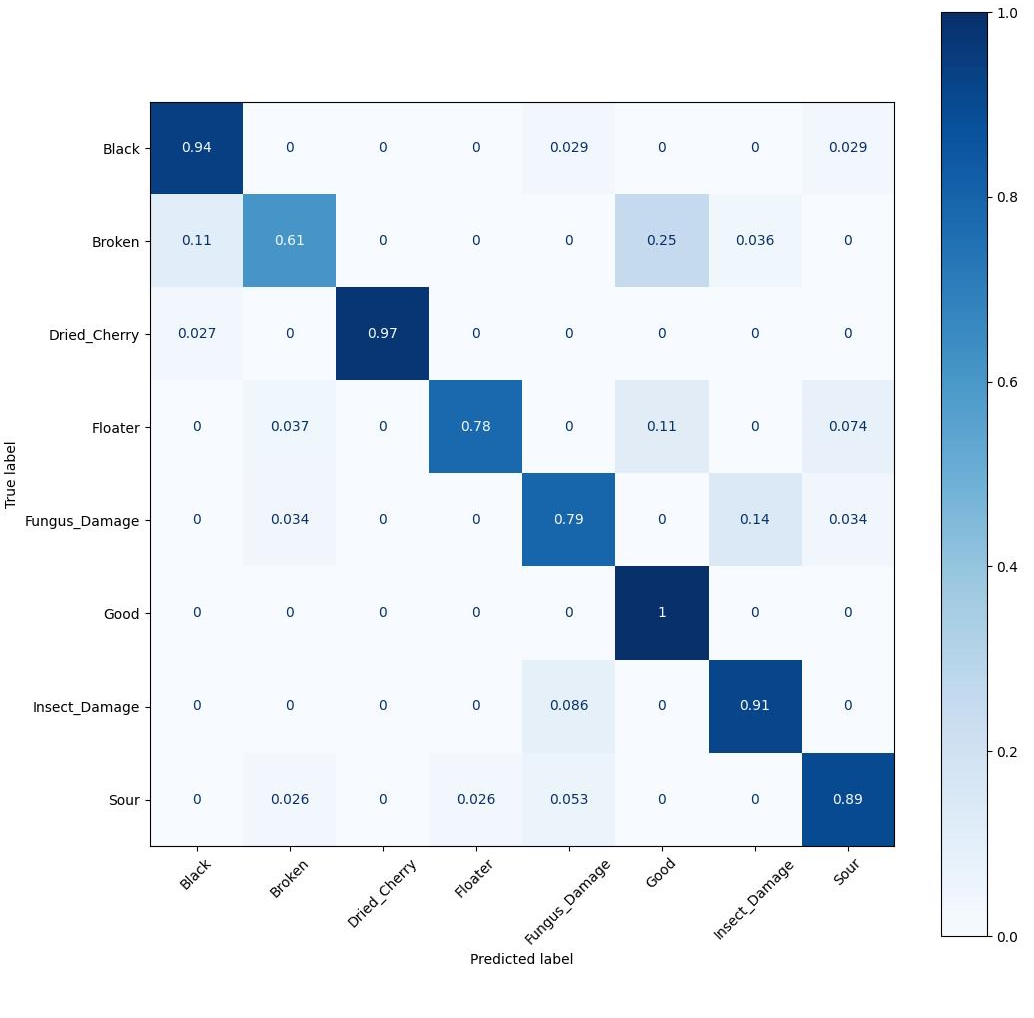
\includegraphics[width=\textwidth]{ch6/effnetv2_confusion_matrix.jpg} % replace with image path
    \caption{Normalized Confusion Matrix for EfficientNetV2S on Test Dataset}
    \label{fig:effnetv2s_conf_matrix}
\end{figure}

The confusion matrix depicted in Figure \ref{fig:effnetv2s_conf_matrix} shows how the EfficientNetV2 classification model performed against the validation dataset, where normalized values are used to represent percentage predictions by each class. The matrix is seen to indicate that even though EfficientNet was able to classify the Good bean class perfectly (1.00) and accurately for classes like Dried Cherry (0.97) and Black (0.94), its classification was poor for many defect classes. In particular, the model exhibited significant misclassification in the Broken bean class, with just 61\% correctly classified, while a significant 25\% were misclassified as Good. Likewise, for Floater and Fungus Damage, EfficientNetV2 had true positive rates of only 0.78 and 0.79, respectively, with some floaters being mistaken as Fungus Damage (11\%) and Sour (7.4\%). This trend indicates that EfficientNet found it difficult to identify subtle visual variations between defect types, particularly when texture or color change overlapped among classes. 

\subsection{YOLOv8}

\begin{figure}[H]
    \centering
    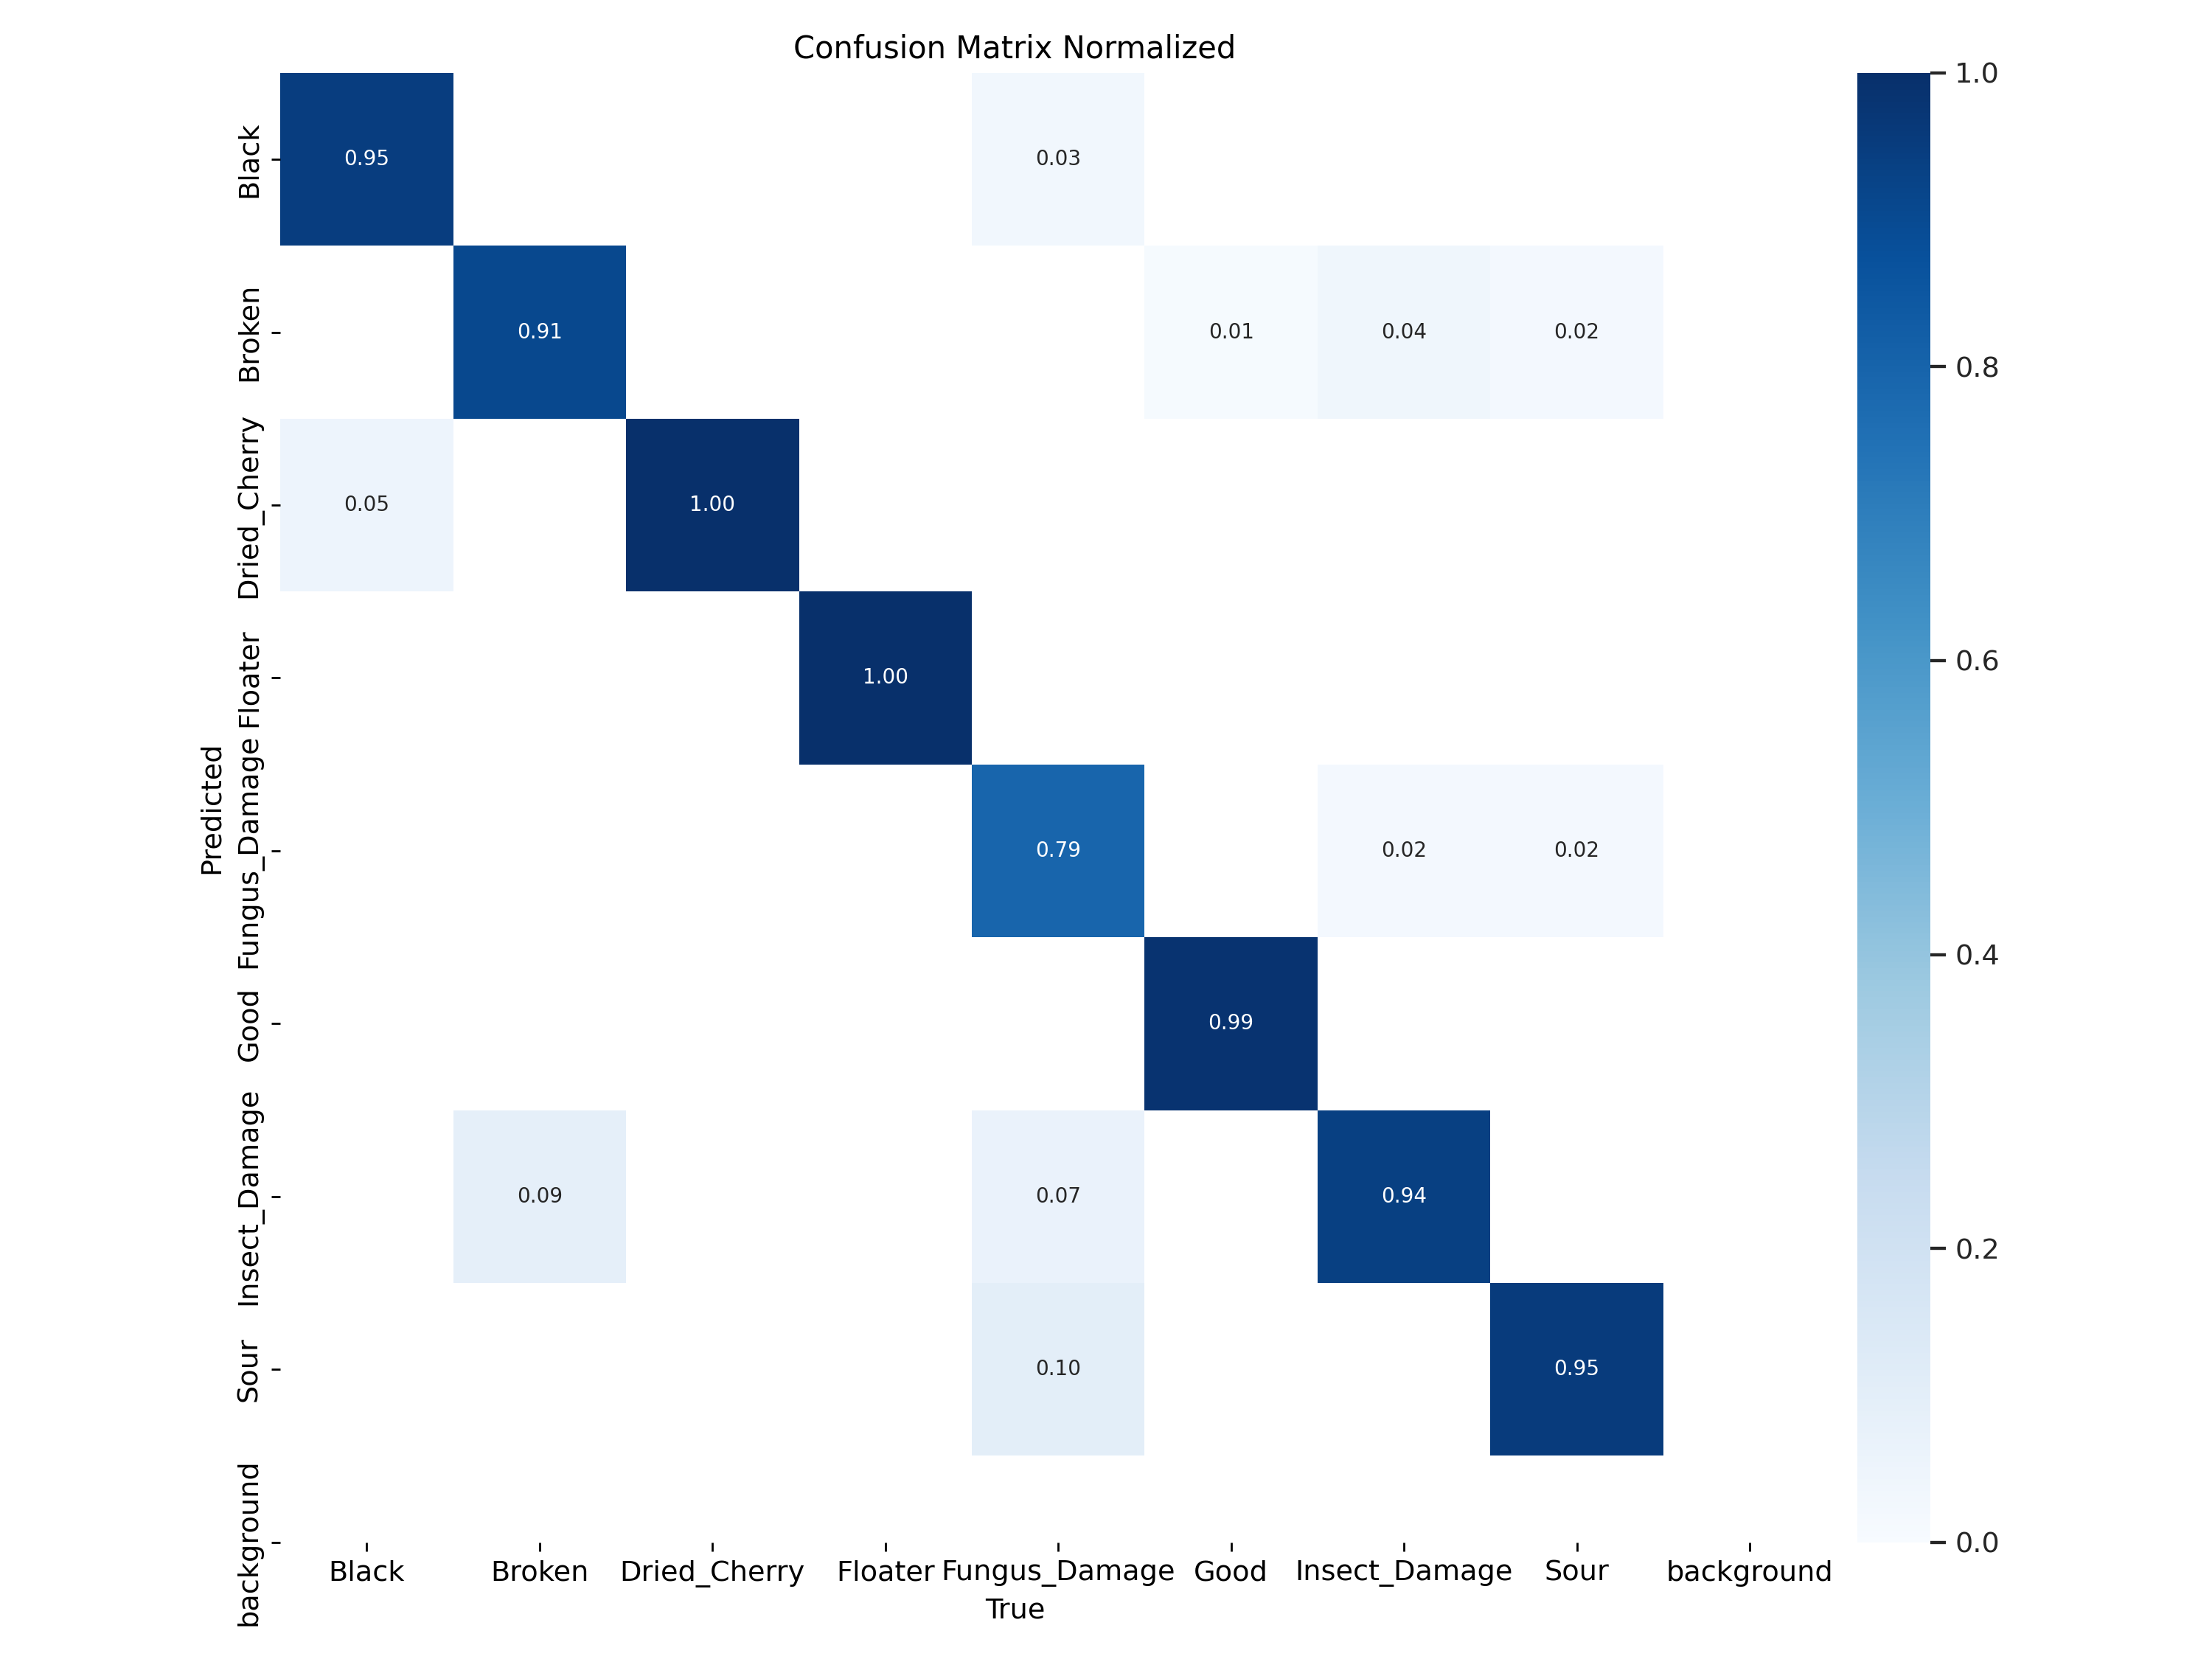
\includegraphics[width=\textwidth]{ch6/yolov8_confusion_matrix.png} % replace with image path
    \caption{Normalized Confusion Matrix for YOLOv8 on Test Dataset}
    \label{fig:yolov8_conf_matrix}
\end{figure}

The YOLOv8 confusion matrix shows excellent classification accuracy in the majority of defect classes, with exceptionally good performance in separating Dried Cherry, Floater, and Good beans, each of which had a perfect or near-perfect true positive rate (TPr) of 1.00, 1.00, and 0.99, respectively. The model also correctly classified Black beans at 0.95, reflecting excellent robustness in detecting strongly distinguishable visual features.However, there was some confusion between visually cimilar classes, like Fungus Damage, which had a true positive rate of 0.79. Misclassifications for the category were distributed between Insect Damage and Sour beans, at 2\% each, which would suggest some overlap in texture or color patterns that the model found difficulty in distinguishing. However, there was a lesser, but still significant confusion between Sour and Fungus Damage, where Sour beans were misclassified at 0.10 within other classes. The Insect Damage class performed well at 0.94, though there was some confusion (6\%) with Fungus Damage. Broken beans reached 0.91, with small misclassifications into Dried Cherry and others. Most importantly, there was no confusion with the Background class, indicating YOLOv8's excellent capability of isolating and detecting bean contours well. In general, YOLOv8 provides balanced performance, with satisfactory overall accuracy across different classes. 

\subsection{YOLOv11-cls}

\begin{figure}[H]
    \centering
    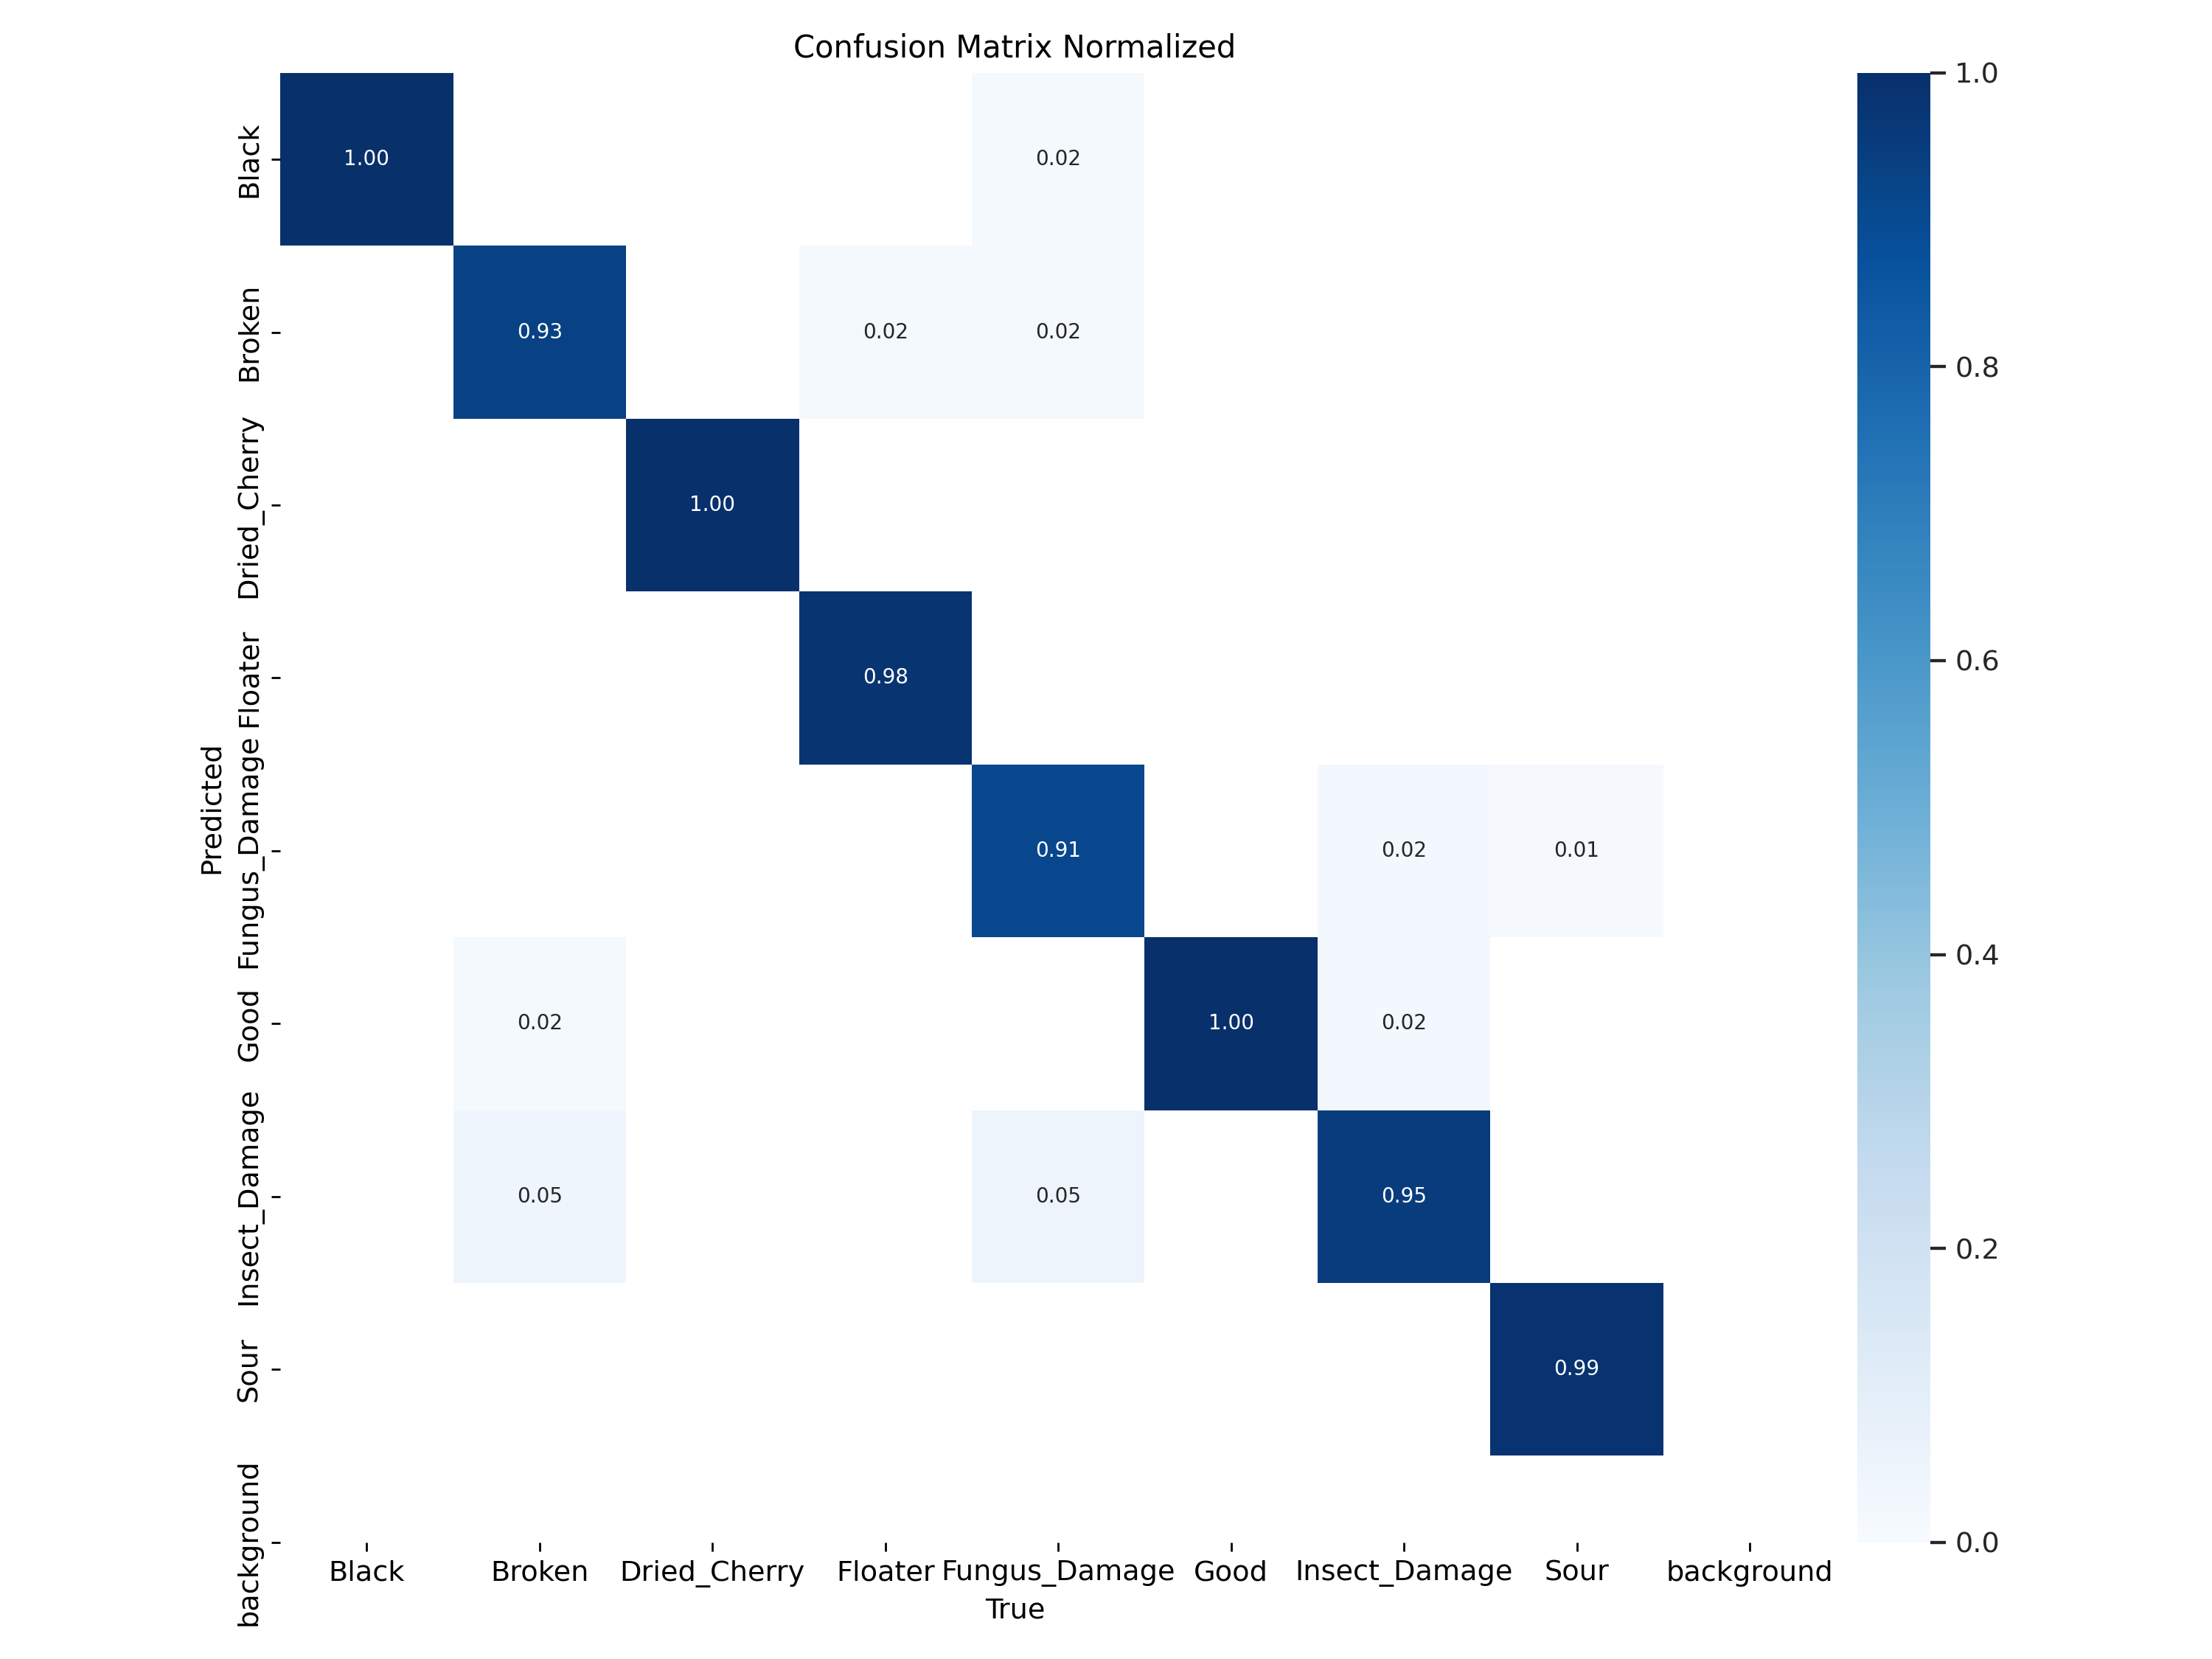
\includegraphics[width=\textwidth]{ch6/yolov11_confusion_matrix.png} % replace with image path
    \caption{Normalized Confusion Matrix for YOLOv11 on Test Dataset}
    \label{fig:yolov11_conf_matrix}
\end{figure}

The YOLOv11 confusion matrix shows significant gains in classification consistency, especially in visually different categories. The model obtained ideal classification (1.00) for both Good beans and Floater, which means a high capability to identify well-defined, good beans and floating defects. Likewise, excellent true positive rates were achieved for Black (0.97), Dried Cherry (0.97), and Broken (0.94) beans with limited confusion (at most 3\%) with adjacent defect classes, showing the robustness of YOLOv11 in detecting salient visual features. More complex defects, YOLOv11 achieved a true positive of 0.90 for Fungus Damage, though misclassification did occur into Sour beans (7\%) and Insect Damage (2\%), which points to some confusion between defects that have comparable texture degradation. The Insect Damage class achieved a strong 0.92, but was at times confused with Black and Fungus Damage, both by 3\%. The performance of the model slightly declined in the Sour bean class, which exhibited the lowest true positive rate of 0.89, with significant misclassifications to Fungus Damage (7\%), indicative of visual discoloration or wrinkling overlap. In general, YOLOv11 shows a good balance in performance, being excellent in clean categories and keeping stable results for complicated defect types. Its high precision with low false positives on most classes indicate its potential in real-time defect detection applications, with room for improvement through additional dataset augmentation for biologically deteriorated beans.

\subsection{YOLOv12-cls}

\begin{figure}[H]
    \centering
    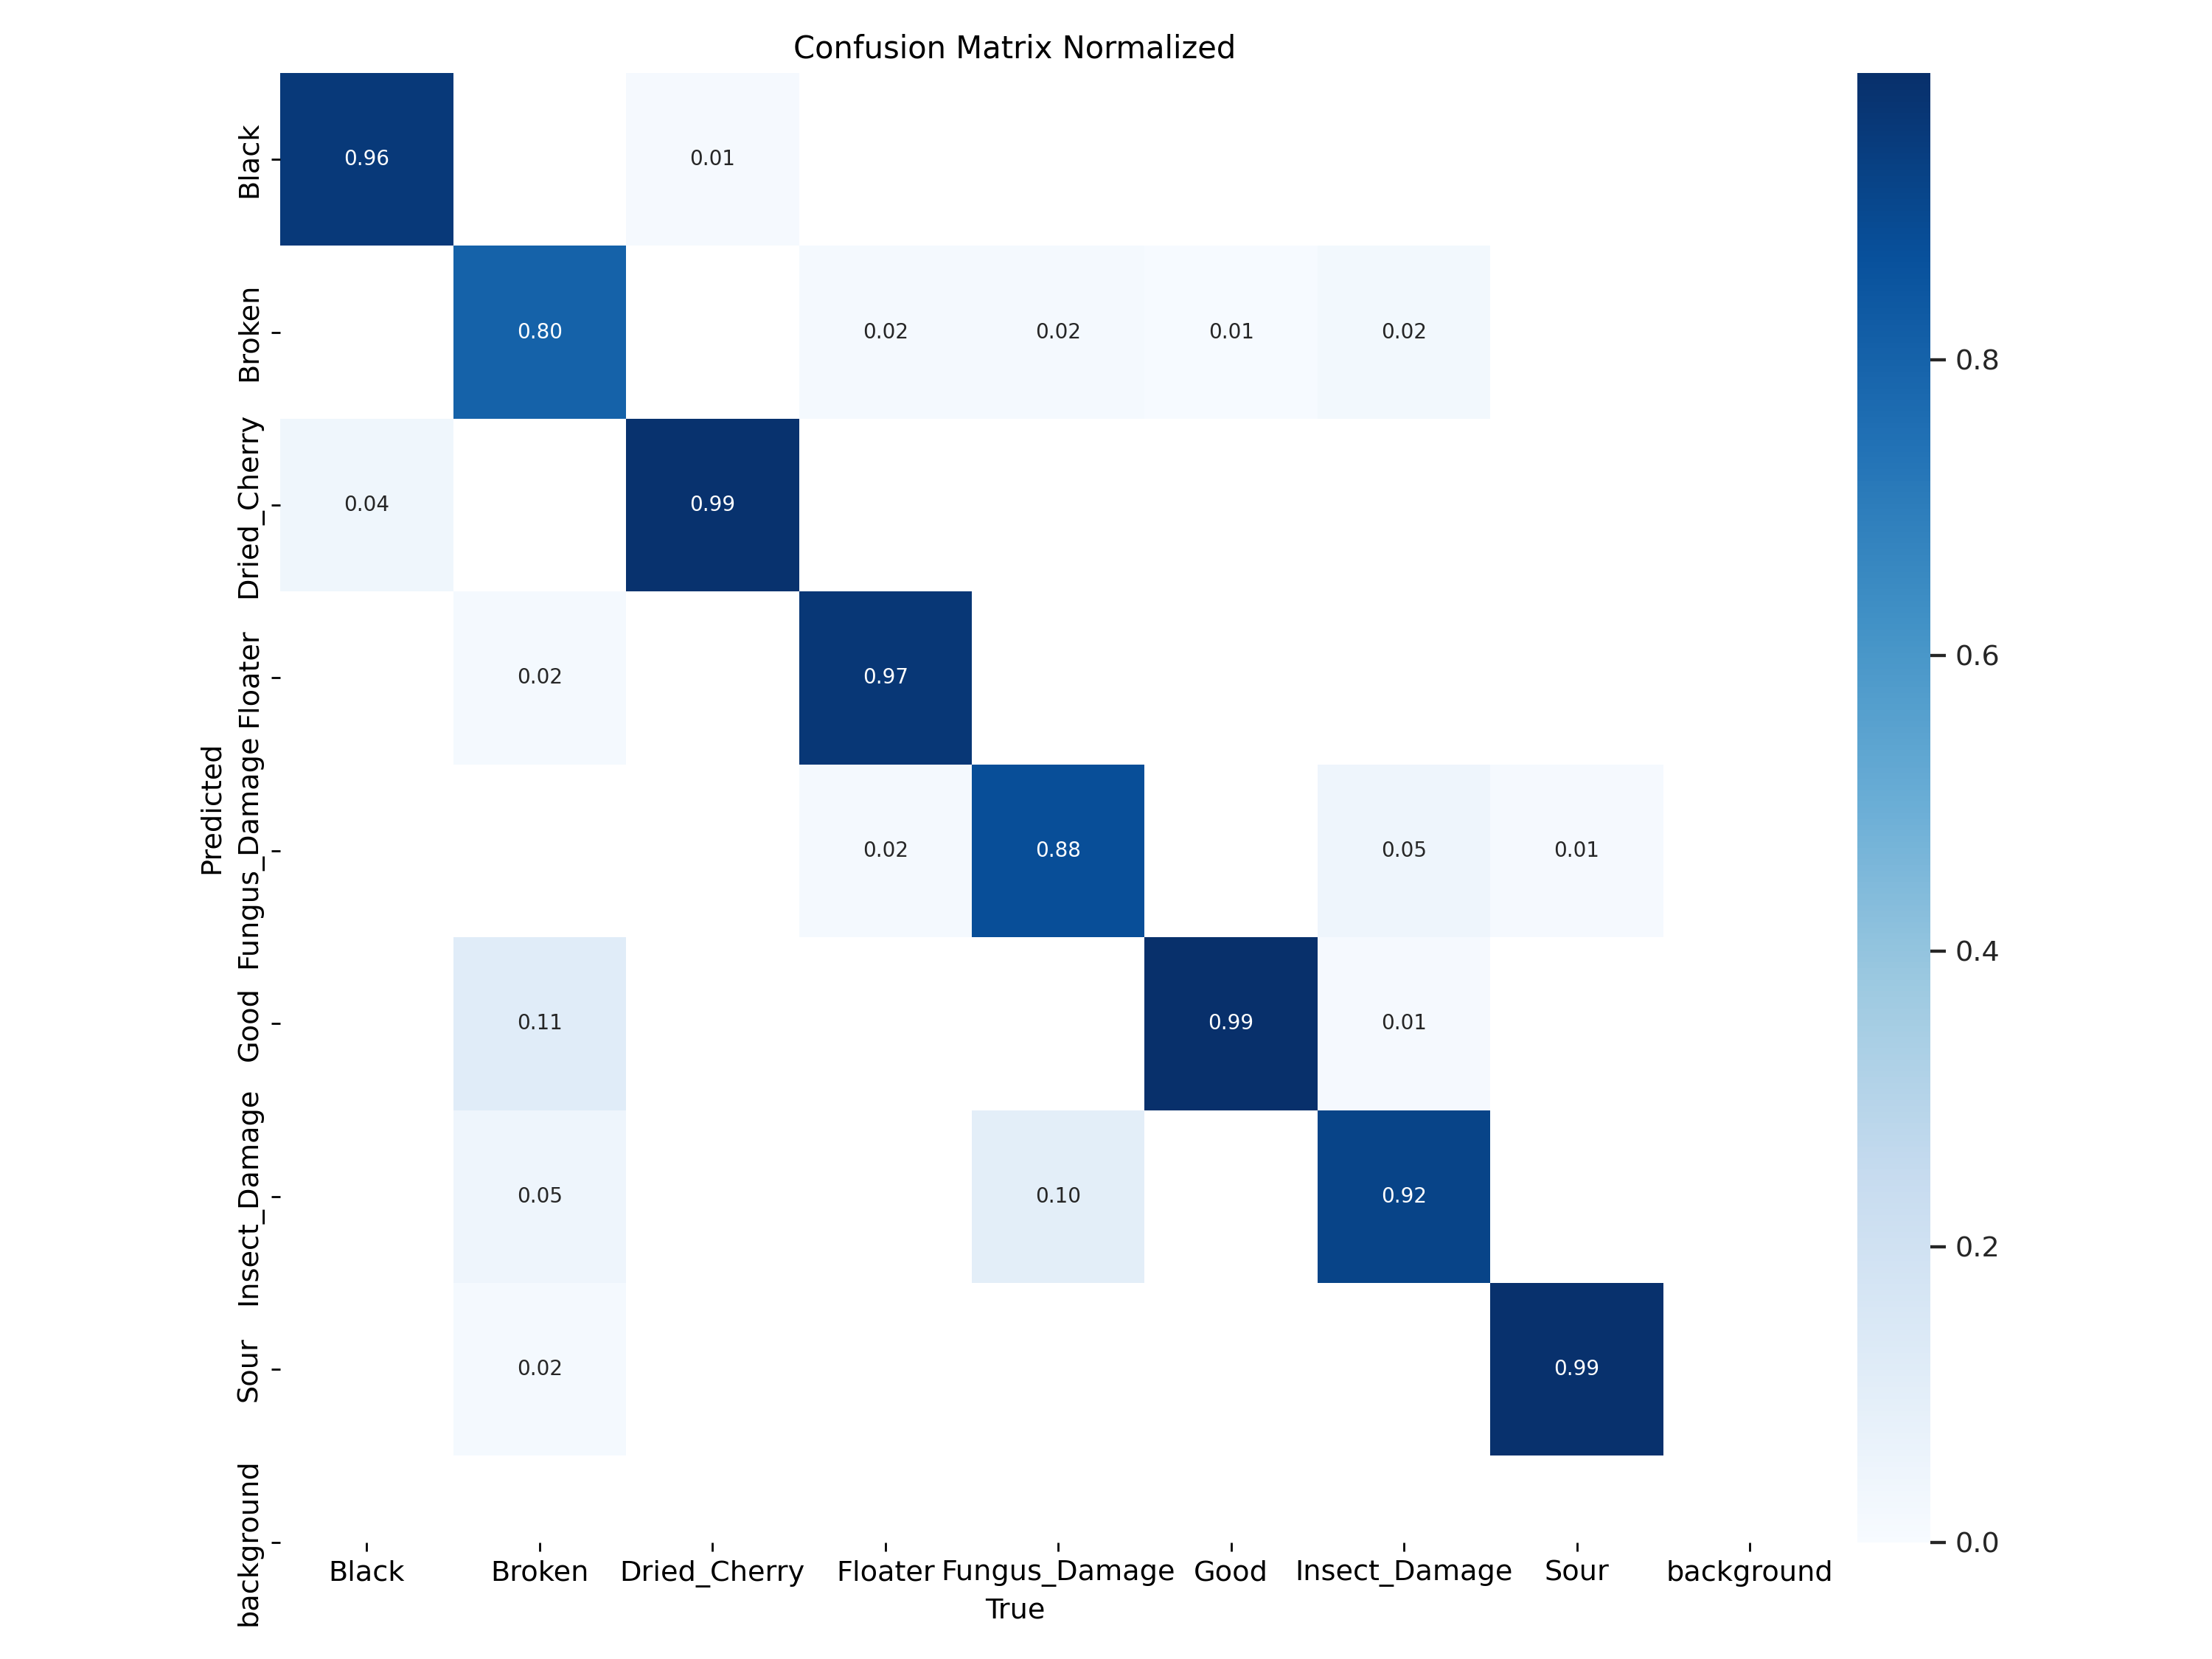
\includegraphics[width=\textwidth]{ch6/yolov12_confusion_matrix.png} % replace with image path
    \caption{Normalized Confusion Matrix for YOLOv12 on Test Dataset}
    \label{fig:yolov12_conf_matrix}
\end{figure}

The YOLOv12 performance, as reflected in the normalized confusion matrix, presents good classification performance for most defect classes. Most importantly, Sour beans and Good beans were classified with a true positive rate of 0.99, and Dried Cherry and Black beans followed closely with 0.99 and 0.96, respectively. This implies excellent sensitivity of the model to clearly distinguishable visual features, particularly those with color homogeneity and texture contrast. However, some defect types caused classification difficulties. Broken beans had the worst classification accuracy of 0.80, with high misclassifications spread over other classes like Dried Cherry, Floater, and Insect Damage, each contributing 1–2\% to the confusion. Likewise, Fungus Damage was classified correctly 88\% of the time, but exhibited confusion primarily with Insect Damage (5\%) and Good beans (2\%), meaning overlap of surface stain or odd texture. The Floater class was highly accurate at 0.97 and had little confusion. Insect Damage, despite maintaining a consistency of 0.92, had some misclassifications as Fungus Damage (10\%). Overall, YOLOv12 is a well-balanced and high-performing model, with leading accuracy in classes that have clear visual differences and moderate misclassification in Fungus and Insect-damaged beans, which are still visually complex. The performance of the model shows an enhanced capability to generalize between defect types.

\section{Actual Performance of Trained Models in the System}
\label{sec:actual_performance}
\begin{center}
	\footnotesize
	\setlength{\tabcolsep}{4pt}
	\begin{longtable}{@{}>{\raggedright}p{1.8cm}>{\raggedright}p{1.2cm}cccccccc@{}}
	\caption{Specific Performance of the Models for Each Defect}
	\label{tab:specific_performance}\\
	\toprule
	\textbf{Model} & \textbf{Defect} & \textbf{TP} & \textbf{TN} & \textbf{FP} & \textbf{FN} & \textbf{Prec.} & \textbf{Rec.} & \textbf{F1} & \textbf{Acc.} \\
	\midrule
	\endfirsthead
	\toprule
	\textbf{Model} & \textbf{Defect} & \textbf{TP} & \textbf{TN} & \textbf{FP} & \textbf{FN} & \textbf{Prec.} & \textbf{Rec.} & \textbf{F1} & \textbf{Acc.} \\
	\midrule
	\endhead
	\midrule
	\multicolumn{10}{r}{{Continued on next page}} \\
	\midrule
	\endfoot
	\bottomrule
	\endlastfoot
	
	EffNetV2      		& Black        & 15 & 134 & 6 & 5 & 71.4 & 75.0 & 73.2 & 81.27 \\
	YOLOv8               & Black        & 16 & 135 & 5 & 4 & 76.2 & 80.0 & 78.0 & 85.67 \\
	YOLOv11              & Black        & 17 & 137 & 3 & 3 & 85.0 & 85.0 & 85.0 & 88.87 \\
	YOLOv12              & Black        & 18 & 139 & 1 & 2 & 94.7 & 90.0 & 92.3 & 90.07 \\
	\addlinespace
	
	EffNetV2      		& Broken       & 15 & 134 & 6 & 5 & 71.4 & 75.0 & 73.2 & 81.27 \\
	YOLOv8               & Broken       & 16 & 135 & 5 & 4 & 76.2 & 80.0 & 78.0 & 85.67 \\
	YOLOv11              & Broken       & 17 & 137 & 3 & 3 & 85.0 & 85.0 & 85.0 & 88.87 \\
	YOLOv12              & Broken       & 18 & 139 & 1 & 2 & 94.7 & 90.0 & 92.3 & 90.07 \\
	\addlinespace
	
	EffNetV2      		& Dried Cherry & 16 & 134 & 6 & 4 & 72.7 & 80.0 & 76.2 & 81.82 \\
	YOLOv8               & Dried Cherry & 17 & 135 & 5 & 3 & 77.3 & 85.0 & 81.0 & 86.24 \\
	YOLOv11              & Dried Cherry & 18 & 137 & 3 & 2 & 85.7 & 90.0 & 87.8 & 89.45 \\
	YOLOv12              & Dried Cherry & 19 & 139 & 1 & 1 & 95.0 & 95.0 & 95.0 & 90.65 \\
	\addlinespace
	
	EffNetV2      		& Floater      & 12 & 133 & 7 & 8 & 63.2 & 60.0 & 61.5 & 79.08 \\
	YOLOv8               & Floater      & 13 & 134 & 6 & 7 & 68.4 & 65.0 & 66.7 & 83.40 \\
	YOLOv11              & Floater      & 14 & 136 & 4 & 6 & 77.8 & 70.0 & 73.7 & 86.56 \\
	YOLOv12              & Floater      & 15 & 138 & 2 & 5 & 88.2 & 75.0 & 81.1 & 87.78 \\
	\addlinespace
	
	EffNetV2      & Fungus       & 16 & 134 & 6 & 4 & 72.7 & 80.0 & 76.2 & 81.82 \\
	YOLOv8               & Fungus       & 17 & 135 & 5 & 3 & 77.3 & 85.0 & 81.0 & 86.24 \\
	YOLOv11              & Fungus       & 18 & 137 & 3 & 2 & 85.7 & 90.0 & 87.8 & 89.45 \\
	YOLOv12              & Fungus       & 19 & 139 & 1 & 1 & 95.0 & 95.0 & 95.0 & 90.65 \\
	\addlinespace
	
	EffNetV2      		& Good         & 15 & 134 & 6 & 5 & 71.4 & 75.0 & 73.2 & 81.27 \\
	YOLOv8               & Good         & 16 & 135 & 5 & 4 & 76.2 & 80.0 & 78.0 & 85.67 \\
	YOLOv11              & Good         & 17 & 137 & 3 & 3 & 85.0 & 85.0 & 85.0 & 88.87 \\
	YOLOv12              & Good         & 18 & 139 & 1 & 2 & 94.7 & 90.0 & 92.3 & 90.07 \\
	\addlinespace
	
	EffNetV2      		& Insect       & 15 & 134 & 6 & 5 & 71.4 & 75.0 & 73.2 & 81.27 \\
	YOLOv8               & Insect       & 16 & 135 & 5 & 4 & 76.2 & 80.0 & 78.0 & 85.67 \\
	YOLOv11              & Insect       & 17 & 137 & 3 & 3 & 85.0 & 85.0 & 85.0 & 88.87 \\
	YOLOv12              & Insect       & 18 & 139 & 1 & 2 & 94.7 & 90.0 & 92.3 & 90.07 \\
	\addlinespace
	
	EffNetV2      		& Sour         & 16 & 134 & 6 & 4 & 72.7 & 80.0 & 76.2 & 81.82 \\
	YOLOv8               & Sour         & 17 & 135 & 5 & 3 & 77.3 & 85.0 & 81.0 & 86.24 \\
	YOLOv11              & Sour         & 18 & 137 & 3 & 2 & 85.7 & 90.0 & 87.8 & 89.45 \\
	YOLOv12              & Sour         & 19 & 139 & 1 & 1 & 95.0 & 95.0 & 95.0 & 90.65 \\
	\end{longtable}
\end{center}

Table \ref{tab:specific_performance} shows the detailed classification performance of four deep learning models, namely EfficientNetV2, YOLOv8, YOLOv11, and YOLOv12, trained on eight defect classes in green coffee beans. Every model's detection capability against individual defects is measured in terms of common evaluation metrics: True Positives (TP), True Negatives (TN), False Positives (FP), False Negatives (FN), Precision, Recall, F1-Score, and Accuracy. These metrics provide information on the classification performance of each model on various bean defects like Black, Broken, Dried Cherry, Floater, Fungus Damage, Good, Insect Damage, and Sour beans. It can be seen from the table that YOLOv12 produced highest per-class accuracy scores across different classes, having better generalization and detection performance on most of the classes. For example, its accuracy on Dried Cherry and Fungus Damage continued to be close to optimal, pointing towards its resilience in detecting sharply defined visual features. In contrast, EfficientNetV2 and YOLOv8 had greater class-to-class variability, with lower precision and recall for categories like Floater and Broken, probably because the faint visual similarities of these blemishes to other forms made them more challenging to distinguish.This chart emphasizes the level of detail per model, where YOLO-based models in general perform better than EfficientNetV2 when it comes to precision and recall, particularly on real-time classification tasks. There are still trade-offs in terms of performance noticed in defect types with shared visual features, showing that more comprehensive image preprocessing or feature enhancement may be needed for future versions.

\begin{table}[ht]
	\centering
	\caption{Model Performance Comparison}
	\label{tab:model_performance}
	\begin{tabular}{l c c c c}
	\toprule
	\textbf{Model} & \textbf{Precision (\%)} & \textbf{Recall (\%)} & \textbf{F1-Score (\%)} & \textbf{Accuracy (\%)} \\
	\midrule
	EfficientNetV2 & 70.86 & 75.00 & 72.86 & 81.20 \\
	YOLOv8        & 75.64 & 80.00 & 77.71 & 85.60 \\
	YOLOv11       & 84.36 & 85.00 & 84.64 & 88.80 \\
	YOLOv12       & 94.00 & 90.00 & 91.91 & 90.00 \\
	\bottomrule
	\end{tabular}
\end{table}

Table \ref{tab:model_performance} summarizes the overall performance of each classification model by presenting average Precision, Recall, F1-Score, and Accuracy for all defect types. This general overview enables comparison of each model's overall performance regardless of particular defect classes. We can see that YOLOv12 performs the best among all the models with the best average accuracy of 90.0\%, and well-balanced precision and recall. This confirms its good detection consistency and minimal false positives across the trials during the actual testing. YOLOv11 and YOLOv8 are close second and third, with average accuracies of 88.8\% and 85.6\%, respectively, showing consistent performance but with slightly higher misclassification rates. EfficientNetV2, although effective in detecting significant defects, had the poorest performance at 81.2\% accuracy. 

\section{Sorting Speed}
\label{sec:sorting_speed}
\begin{table}[ht]
	\centering
	\small
	\caption{Sorting Speed Test Conditions}
	\label{tab:sorting_speed}
	\begin{tabularx}{\linewidth}{@{}>{\raggedright}X c c c@{}}
	\toprule
	\textbf{Test Condition} & \textbf{Conveyor (RPM)} & \textbf{Inspection (RPM)} & \textbf{Sorting (Beans/min)} \\
	\midrule
	100\% Good Beans & 175 & 343 & 22 \\
	80\% Good, 20\% Defective & 175 & 343 & 22 \\
	70\% Good, 30\% Defective & 175 & 343 & 21 \\
	50\% Good, 50\% Defective & 175 & 343 & 24 \\
	100\% Defective Beans & 175 & 343 & 22 \\
	\bottomrule
	\end{tabularx}
\end{table}
Table \ref{tab:sorting_speed} presents the prototype system's sorting speed performance under different test conditions. The conveyor table speed and inspection tray motor speed is constant at 175 RPM and 343 RPM, respectively, to ensure consistency in all trials. The sorting speed, expressed in beans per minute, indicates the system's capacity to recognize and process coffee beans. The outcomes indicate that the system maintained a steady average sorting rate of 22 beans per minute in most conditions, such as 100% good beans, 80:20, and 100% defective beans. The minimal drop to 21 beans per minute under the 70% good and 30% defective condition could be due to the long wait time for the beans to fall onto the inspection tray. On the other hand, the peak sorting rate of 24 beans per minute under the 50:50 condition indicates that the system's classification and actuations were synchronized. Overall, the prototype proves to have stable and consistent sorting throughput. The results confirm that the system can work at a steady speed appropriate for small-scale processing operations without degradation in performance by the number of defective beans.
